\documentclass[conference]{IEEEtran}
\usepackage{amsmath,amssymb}
\usepackage{graphicx}
\usepackage{booktabs}
\usepackage{tikz}
\usetikzlibrary{positioning,fit,backgrounds}
\usepackage{url}
\usepackage{cite}
\usepackage{subcaption}
\usepackage{balance}

\begin{document}

\title{Generalization Gap and Adaptive Retraining in Machine Learning-Based\\
Network Intrusion Detection: A Live-Traffic Case Study with XGBoost}

\author{
\IEEEauthorblockN{Brindha Adiga}
\IEEEauthorblockA{Computer Science and Engineering\\
Global Academy Of Technology\\
Bangalore, India\\
brindhaadiga1ga23cs030@gmail.com}
\and
\IEEEauthorblockN{Deepa MJ}
\IEEEauthorblockA{Computer Science and Engineering\\
Global Academy Of Technology\\
Bangalore, India\\
deepamj1ga23cs035@gmail.com}
\and
\IEEEauthorblockN{MT Yashas}
\IEEEauthorblockA{Computer Science and Engineering\\
Global Academy Of Technology\\
Bangalore, India\\
mtyashas1ga23cs091@gmail.com}
\and
\IEEEauthorblockN{Nikita Chavan}
\IEEEauthorblockA{Computer Science and Engineering\\
Global Academy Of Technology\\
Bangalore, India\\
nikitachavan1ga23cs111@gmail.com}
\and
\IEEEauthorblockN{Prof. Sowmya BK}
\IEEEauthorblockA{Computer Science and Engineering\\
Global Academy Of Technology\\
Bangalore, India\\
sowmya.bk@gat.ac.in}
}

\maketitle

\begin{abstract}
Machine-learning intrusion detection systems (ML-IDS) routinely report
95--99\% accuracy on benchmark datasets, yet this accuracy is known to
collapse once a model is evaluated on a different dataset -- a
cross-dataset generalization gap. This work extends that problem to a
harder, unstudied axis: from a static benchmark to traffic physically
captured live on the network being protected. Using an XGBoost-based IDS
trained to 99.69\% accuracy (99.99\% ROC-AUC) on CIC-IDS-2017, we show live
lab traffic first collapsed in ranking to near-chance (ROC-AUC 0.61)
despite acceptable raw accuracy, was restored to 99.95\% via a
ground-truth-informed adaptive retrain, then partially failed again on a
larger, more diverse capture (95.16\% accuracy, all unseen-port traffic
misclassified) before a second targeted retrain closed the gap (99.74\%),
after fixing three dormant retraining-pipeline defects. Benchmark accuracy
is not a reliable proxy for live deployment readiness, and one retrain does
not permanently close the gap as traffic diversity grows.
\end{abstract}

\renewcommand{\IEEEkeywordsname}{Keywords}
\begin{IEEEkeywords}
live traffic evaluation, domain generalization, adaptive retraining, intrusion detection, XGBoost
\end{IEEEkeywords}

\section{Introduction}

Machine-learning-based intrusion detection systems are almost universally
evaluated the same way: train and test on splits of the same static,
pre-captured benchmark dataset, most commonly CIC-IDS-2017 or its 2018
successor. This produces impressive numbers -- accuracies above 99\% are
routine -- but says little about how such a system behaves once deployed
against traffic it was never shown during training.

Cantone \textit{et al.}~\cite{cantone2024crossdataset} put a number on part
of this problem: when several flow-based classifiers trained on
CIC-IDS-2017 are scored against CSE-CIC-IDS-2018 instead of their own
held-out split, recall falls sharply even though the model architecture
itself never changes -- evidence that what gets learned is tied to
artifacts of a particular data collection rather than to attack behavior
that transfers. This paper pushes past an axis that kind of comparison
cannot reach: two static datasets are still, in the end, two curated
corpora. We instead take a trained model and point it at traffic
physically captured, in real time, from the network it is supposed to be
protecting, and find the same collapse there too -- worse than the
dataset-to-dataset case -- and that it comes back on a second, more varied
capture even after an initial fix appeared to work. We study these
findings on SENTINEL, our own 13-phase, 32-module machine-learning-based
intrusion prevention framework (Section~\ref{sec:architecture}); we refer
to it as SENTINEL throughout the rest of this paper.

Our contributions are:
\begin{enumerate}
\item We reproduce the cross-dataset generalization collapse on our own
      XGBoost + ANOVA-feature-selection pipeline, consistent with
      \cite{cantone2024crossdataset}, and confirm that combined-dataset
      training resolves it, matching prior findings.
\item We provide, to our knowledge, the first empirical characterization of
      the dataset-to-live-traffic generalization gap, using a physical
      lab with ground-truth-labelled packet captures rather than a
      simulated or synthetic distribution shift.
\item We diagnose three previously dormant implementation defects in the
      adaptive-retraining pipeline used to close the gap -- a systems
      finding alongside the machine-learning one, since the correction
      mechanism itself first had to be debugged before it could be
      trusted.
\item We show the gap is not closed permanently by a single retrain: a
      larger, more diverse live capture re-exposes it along a dimension
      (destination port) the first correction never generalized across,
      motivating diversity-aware validation over one-shot correction.
\end{enumerate}

This paper deliberately scopes to SENTINEL's core ML detection pipeline
and the generalization-gap findings above rather than its full feature set
(Section~\ref{sec:architecture}). The remainder of
this paper is organized as follows. Section~\ref{sec:related} reviews
related work on cross-dataset and temporal generalization in ML-IDS.
Section~\ref{sec:architecture} briefly describes the system architecture.
Section~\ref{sec:methodology} details the datasets, pipeline, and
experimental design. Section~\ref{sec:results} presents the three
escalating findings. Section~\ref{sec:discussion} discusses their
implications and limitations, and Section~\ref{sec:conclusion} concludes.

\section{Related Work}
\label{sec:related}

The CIC-IDS-2017 dataset~\cite{sharafaldin2018generating} and its
CSE-CIC-IDS-2018 successor remain the dominant benchmarks for ML-IDS
research, collected via the same methodology (real background traffic
plus scripted attacks in a controlled testbed, flow features extracted via
CICFlowMeter). Most published work reports accuracy on held-out splits of
a single such dataset -- a concern raised as early as
Viegas \textit{et al.}~\cite{viegas2017reliable}, who argued that
anomaly-based detectors rarely reach real-world deployment precisely
because evaluation methodology does not account for production-network
properties; that concern predates CIC-IDS-2017 as the field's standard
benchmark and, as this paper shows, remains only partly addressed by it.
Even recent work stays within this static-evaluation pattern:
Thanh~\cite{thanh2026tanids} proposes a deployment-\emph{oriented}
evaluation framework (in-dataset, cross-dataset, mixed-domain, and
limited-label fine-tuning scenarios) that nonetheless conducts every
experiment on historical records from two existing benchmark corpora
rather than on traffic a network actually produced, and
Layeghy and Portmann~\cite{layeghy2023explainable} likewise confine their
explainability-driven cross-domain analysis to dataset pairs (UNSW-NB15,
CIC-IDS, KDD99) rather than live capture.

The clearest existing evidence for the gap this paper reproduces comes
from Cantone \textit{et al.}~\cite{cantone2024crossdataset}: across
several flow-based classifier architectures, moving the evaluation set
from one CIC-family corpus to another causes recall to fall far faster
than overall accuracy does, even though each model still looks nearly
perfect when scored against the data it was trained on.
Section~\ref{sec:results} reproduces that exact pattern on our own
pipeline before pushing the comparison further. A separate line of work
by Zouhri \textit{et al.}~\cite{zouhri2024filter} compares several
univariate and multivariate feature-selection filters -- among them the
ANOVA F-value criterion this pipeline also relies on -- across
CIC-IDS-2017, CSE-CIC-IDS-2018, and CIC-ToN-IoT, giving independent
support for ANOVA selection as a deliberate rather than arbitrary choice
within this pipeline family (Section~\ref{sec:methodology}). Elangovan
\textit{et al.}~\cite{elangovan2026temporal} approach a related question
from a different angle -- time rather than deployment context -- and find
that classifiers trained on 2017 enterprise traffic lose
${\Delta}$F1${\approx}$0.20--0.27 when applied years later to IoT traffic
collected in 2023--2024; that temporal axis of the gap is complementary
to, and outside the scope of, the live-deployment axis this paper studies.
A third strand of related work targets adaptation directly rather than
measuring the gap itself: Gupta \textit{et al.}~\cite{gupta2025generative}
combine selective sample annotation with synthetic data generation to
correct for concept drift and class imbalance in streaming intrusion
detection; Section~\ref{sec:discussion} contrasts that more elaborate
correction strategy against the considerably simpler one used here.

What none of these three studies do -- comparing datasets to each other,
comparing datasets across time, or correcting for drift within a single
dataset -- is compare a benchmark-trained model against traffic a real
network actually produced. That is the gap this paper fills: the same
collapse these studies document reappears, more severely, the moment a
model leaves curated data behind entirely, and, novel here, a single
corrective retrain does not close it for good -- it resurfaces as the
live traffic observed grows more varied.

\section{System Architecture}
\label{sec:architecture}

SENTINEL (Fig.~\ref{fig:architecture}) ingests packets, flows, and logs,
enriches them with threat-intelligence signals (IP/domain reputation, Tor
exit nodes, honeypot alerts), and passes both into a three-layer Detection
Engine: an XGBoost-based flow classifier (the subject of this paper), a
signature-based layer matching known payload patterns (SQL injection, XSS,
command injection, web shells, CSRF), and an Isolation-Forest-based anomaly
detector for zero-day traffic. Detections fan out to attribution (MITRE
ATT\&CK~\cite{mitreattack} mapping, geolocation, threat-actor profiling),
response (IP blacklisting, connection termination, rate limiting),
adaptive retraining, forensics (PCAP logging, timeline reconstruction), and
SHAP-based explainability, all surfaced on a live dashboard. This paper
evaluates only the ML classification layer of the Detection Engine; the
remaining layers are named here for context but are outside its scope,
except where the adaptive-retraining loop is directly implicated in
Section~\ref{sec:discussion}, and where SHAP explainability is applied
directly to this layer's classifier in Section~\ref{sec:results}.D.

\begin{figure}[b]
\centering
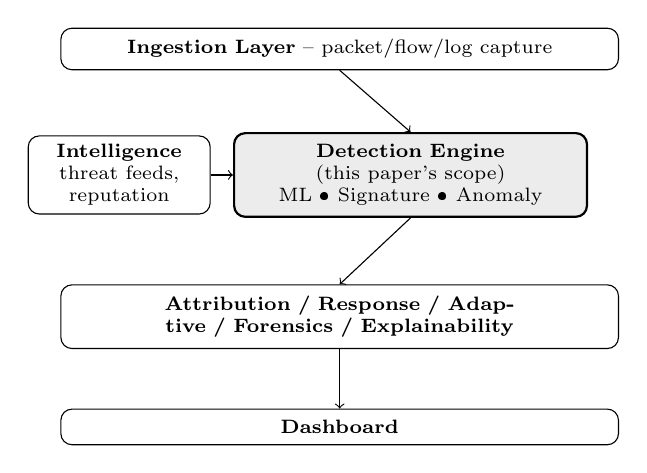
\begin{tikzpicture}[
  layer/.style={draw, rounded corners, align=center, font=\scriptsize, inner sep=4pt},
  scoped/.style={draw, thick, rounded corners, align=center, font=\scriptsize, inner sep=4pt, fill=gray!15},
  small/.style={draw, rounded corners, align=center, font=\scriptsize, inner sep=3pt}
]
\node[layer, text width=6.8cm] (ingest) at (3.5,6)
  {\textbf{Ingestion Layer} -- packet/flow/log capture};

\node[small, text width=2.1cm] (intel) at (0.7,4.4)
  {\textbf{Intelligence}\\threat feeds, reputation};

\node[scoped, text width=4.2cm] (detect) at (4.4,4.4)
  {\textbf{Detection Engine}\\(this paper's scope)\\ML \textbullet\ Signature \textbullet\ Anomaly};

\node[layer, text width=6.8cm] (down) at (3.5,2.6)
  {\textbf{Attribution / Response / Adaptive / Forensics / Explainability}};

\node[layer, text width=6.8cm] (dash) at (3.5,1.2)
  {\textbf{Dashboard}};

\draw[->] (ingest.south) -- (detect.north);
\draw[->] (intel.east) -- (detect.west);
\draw[->] (detect.south) -- (down.north);
\draw[->] (down.south) -- (dash.north);
\end{tikzpicture}
\caption{SENTINEL system architecture (compact). This paper evaluates
only the highlighted Detection Engine; the other layers of the deployed
32-module system are shown for context, except where the Adaptive layer's
retraining pipeline is directly implicated in the defects discussed in
Section~\ref{sec:discussion}.}
\label{fig:architecture}
\end{figure}

\section{Methodology}
\label{sec:methodology}

\subsection{Datasets}
We use four datasets, two static benchmarks and two live packet captures
of our own. CIC-IDS-2017~\cite{sharafaldin2018generating} (2{,}636{,}647
flows, 82 features, five days of labelled traffic covering DoS, DDoS,
brute force, web attacks, infiltration, port scanning, and botnet
activity) is the training set throughout. Its successor CSE-CIC-IDS-2018
(15{,}007{,}575 flows, 80 features, extended attack scenarios on a larger
AWS-hosted topology) is used only as the cross-dataset evaluation target
in Section~\ref{sec:results}.A. \emph{Live Capture 1} (2{,}092 flows:
2{,}038 attacker, 54 benign) and \emph{Live Capture 2} (17{,}612 flows:
15{,}247 attacker, 2{,}365 benign) are ground-truth-labelled packet
captures we generated ourselves from the VirtualBox lab described in
Section~\ref{sec:methodology}.C, using known source IPs and controlled
attacker tooling (\texttt{nmap}, \texttt{hydra}) rather than any existing
public corpus; these are the evaluation targets for
Sections~\ref{sec:results}.B and~\ref{sec:results}.C respectively.

\subsection{Feature Pipeline}
All experiments use the same pipeline: median imputation, standard
scaling, ANOVA F-value feature selection (\texttt{SelectKBest}, $k=30$)
following the validated use of this selection family on the same dataset
pair~\cite{zouhri2024filter}, and an XGBoost~\cite{chen2016xgboost}
classifier ($n_{\text{estimators}}{=}500$, $\text{max\_depth}{=}8$,
$\text{learning\_rate}{=}0.05$, $\text{subsample}{=}0.8$,
$\text{colsample\_bytree}{=}0.8$, $\text{random\_state}{=}42$).

\subsection{Experimental Design}
Three experiments correspond to the three findings of
Section~\ref{sec:results}: (i) train on CIC-IDS-2017, evaluate on
CSE-CIC-IDS-2018, versus combined-dataset training; (ii) evaluate the
CIC-IDS-2017-trained model against traffic physically captured in a
VirtualBox-based lab (an attacker host at \texttt{192.168.56.10} running
\texttt{nmap}/\texttt{hydra}, a benign-traffic host at
\texttt{192.168.56.20}, and the protected host running live packet
capture via Scapy/Npcap and a custom flow collector re-implementing
CICFlowMeter's feature set); (iii) re-evaluate the corrected model from
(ii) against a second, independently generated, larger and more diverse
live capture.

\subsection{Adaptive Retraining Strategy}
Both live-traffic corrections mix the \emph{entire} ground-truth-labelled
capture into retraining, rather than only the model's misclassified rows,
weighted alongside a baseline sample of the original CIC-IDS-2017
training distribution. Retraining only on mistakes risks silently
regressing flow shapes the model already classified correctly, since they
would otherwise have zero representation in the retrain; mixing in the
full capture at baseline weight preserves them.

\subsection{Evaluation Metrics}
We report accuracy, precision, recall, F1-score, ROC-AUC, and the full
confusion matrix for every experiment. This is a deliberate methodological
choice, not a formality: Section~\ref{sec:results} shows a case where
accuracy alone (98.66\%) looks acceptable while ROC-AUC (0.61) reveals the
model's ranking is barely better than chance -- accuracy alone is
misleading precisely when the two classes are imbalanced, which live
traffic captures typically are.

\section{Results}
\label{sec:results}

\subsection{Cross-Dataset Domain Shift}

\begin{table}[t]
\centering
\caption{In-distribution benchmark (CIC-IDS-2017 $\rightarrow$ CIC-IDS-2017)}
\label{tab:table1}
\begin{tabular}{lr}
\toprule
Metric & Value \\
\midrule
Accuracy & 99.69\% \\
Precision & 98.53\% \\
Recall & 99.68\% \\
F1-score & 99.10\% \\
ROC-AUC & 99.99\% \\
TP / TN / FP / FN & 90{,}018 / 435{,}681 / 1{,}344 / 287 \\
Flows tested & 527{,}330 \\
\bottomrule
\end{tabular}
\end{table}

Table~\ref{tab:table1} establishes the in-distribution ceiling our model
achieves under standard held-out evaluation -- the number every subsequent
comparison in this paper is measured against. We independently reproduced
this result via a fresh full-dataset retrain, obtaining 99.79\% accuracy,
99.20\% precision, 99.57\% recall, 99.39\% F1, and 99.99\% ROC-AUC, within
noise of the values above.

\begin{table}[t]
\centering
\caption{Cross-dataset shift vs. combined training}
\label{tab:table2}
\begin{tabular}{lrr}
\toprule
Metric & 2017$\rightarrow$2018 & 2017+2018$\rightarrow$2018 \\
\midrule
Accuracy & 85.64\% & --- \\
Precision & 74.18\% & 100.00\% \\
Recall & 20.12\% & 80.83\% \\
F1-score & 31.66\% & 89.40\% \\
ROC-AUC & 92.35\% & --- \\
Flows tested & 15{,}188{,}468 & --- \\
\bottomrule
\end{tabular}
\end{table}

Table~\ref{tab:table2} and Fig.~\ref{fig:finding1} show the cross-dataset
collapse: a model trained on CIC-IDS-2017 and evaluated on
CSE-CIC-IDS-2018 retains 85.64\% accuracy -- an artifact of class
imbalance -- while recall collapses to 20.12\%. This mirrors the collapse
Cantone \textit{et al.}~\cite{cantone2024crossdataset} report for the same
dataset pair, replicated here on our own pipeline. Training on the
combined 2017+2018 corpus resolves it: recall rises to 80.83\% and
precision to 100.00\%, consistent with \cite{cantone2024crossdataset}'s
finding that the gap is a dataset-artifact problem rather than an
inherent limit of flow-based classification.

\begin{figure}[t]
\centering
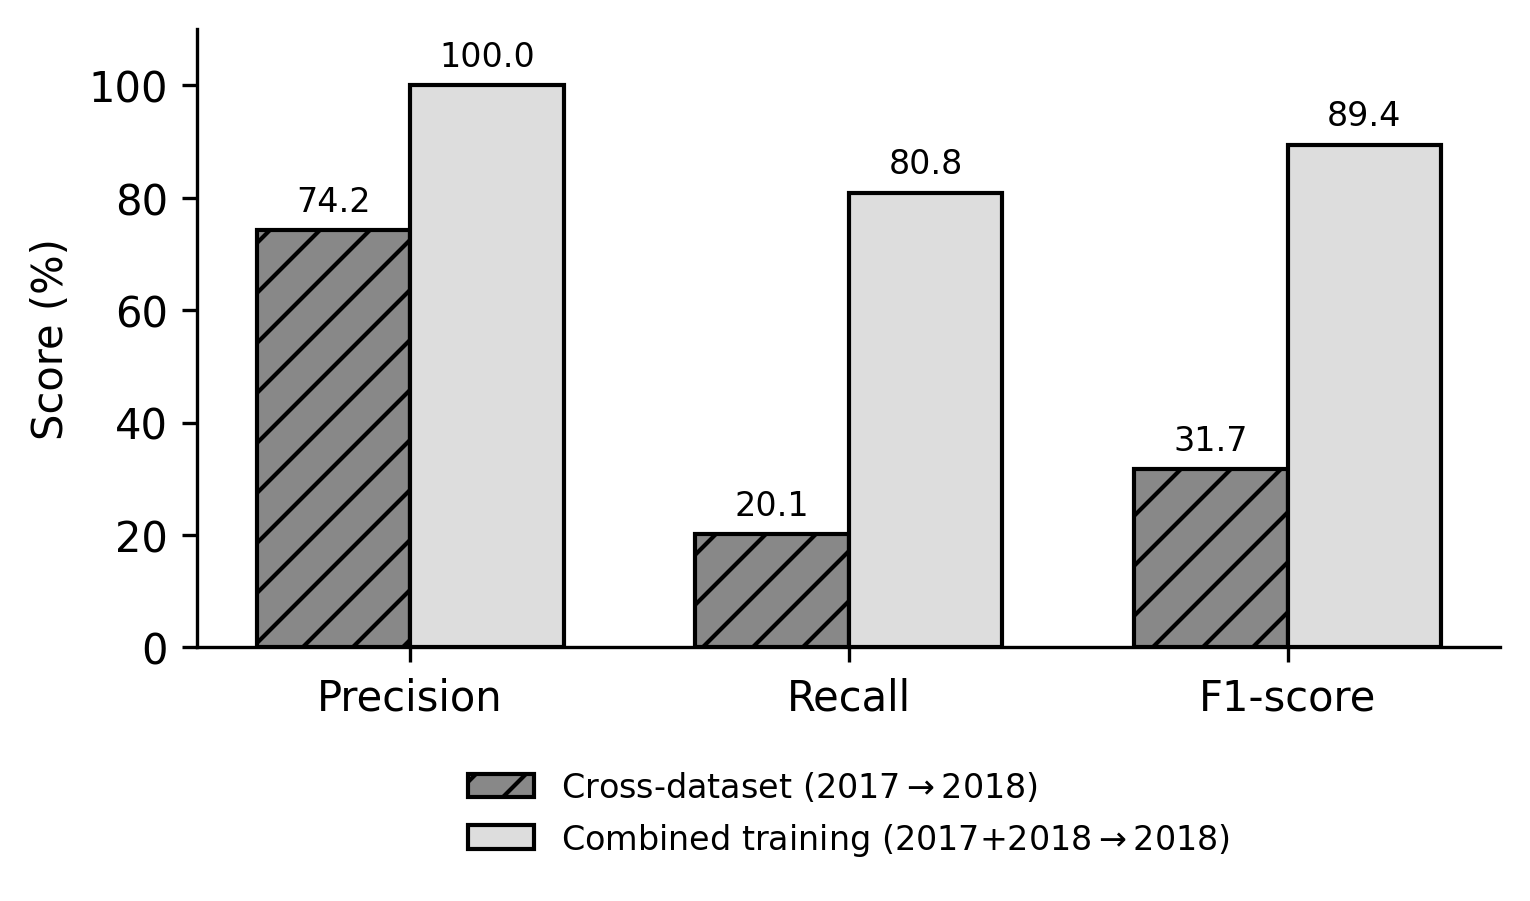
\includegraphics[width=0.9\linewidth]{figures/finding1_bar_2017v2018.png}
\caption{Cross-dataset shift (2017$\rightarrow$2018) vs. combined training, precision/recall/F1.}
\label{fig:finding1}
\end{figure}

\subsection{Dataset-to-Live Collapse}

The same 99.69\%-accuracy model was evaluated against traffic physically
captured live in our lab (2{,}092 flows: 2{,}038 attacker, 54 benign,
ground truth from known source IPs). Table~\ref{tab:table3} reports a
same-session reproducibility check against this capture, which we treat as
the anchor result since it carries a full confusion matrix and ROC curve;
an earlier session reported an even lower pre-fix accuracy of 1.29\% on
this same capture, which we report here for completeness but did not
independently re-verify in this pass.

\begin{table}[t]
\centering
\caption{Dataset-to-live collapse and adaptive-retrain correction}
\label{tab:table3}
\begin{tabular}{lrr}
\toprule
Metric & Before retrain & After retrain \\
\midrule
Accuracy & 98.66\% & 99.95\% \\
Precision & 98.69\% & 100.00\% \\
Recall & 99.95\% & 99.95\% \\
F1-score & 99.32\% & 99.98\% \\
ROC-AUC & \textbf{0.6086} & \textbf{0.9999} \\
TP / TN / FP / FN & 2037/27/27/1 & 2037/54/0/1 \\
\bottomrule
\end{tabular}
\end{table}

The headline result here is not the accuracy figure but the ROC-AUC gap
(Fig.~\ref{fig:finding2grid}): 98.66\% accuracy looks deceptively
acceptable, but a ROC-AUC of 0.61 shows the underlying ranking was barely
better than random -- exactly half of
real benign traffic (27 of 54 flows) was misclassified as an attack. Both
misclassified flows (Fig.~\ref{fig:m4confidence}) were far more minimal
than anything in CIC-IDS-2017's training distribution: a benign HTTP
request (7 forward / 5 backward packets, 6--15\,ms) and a single SYN probe
(1/1 packets, 9--36\,\textmu s) -- both too sparse to resemble the model's
learned notions of "typical benign" or "typical PortScan." An adaptive
retrain mixing the full ground-truth-labelled capture into training
(Section~\ref{sec:methodology}) restored ROC-AUC to 0.9999 and eliminated
all 27 false positives.

\subsection{Gap Persists Within Live Traffic}

The corrected model from Section~\ref{sec:results}.B was re-evaluated
against a second, independently generated, larger live capture (17{,}612
flows: 15{,}247 attacker, 2{,}365 benign; a new benign host, an
\texttt{nmap -sS -p 1-10000} scan, and 2{,}000 varied HTTP requests
including 732 deliberate probes to a destination port -- 8081 -- absent
from the first capture).

\begin{table}[t]
\centering
\caption{Gap re-opening on a larger, more diverse capture}
\label{tab:table4}
\begin{tabular}{lrr}
\toprule
Metric & Before 2nd retrain & After 2nd retrain \\
\midrule
Accuracy & 95.16\% & 99.74\% \\
Precision & 95.38\% & 100.00\% \\
Recall & 99.22\% & 99.70\% \\
F1-score & 97.26\% & 99.85\% \\
ROC-AUC & 0.8987 & 0.9998 \\
TP / TN / FP / FN & 15128/1632/733/119 & 15201/2365/0/46 \\
\bottomrule
\end{tabular}
\end{table}

\begin{figure}[t]
\centering
\begin{subfigure}{0.23\textwidth}
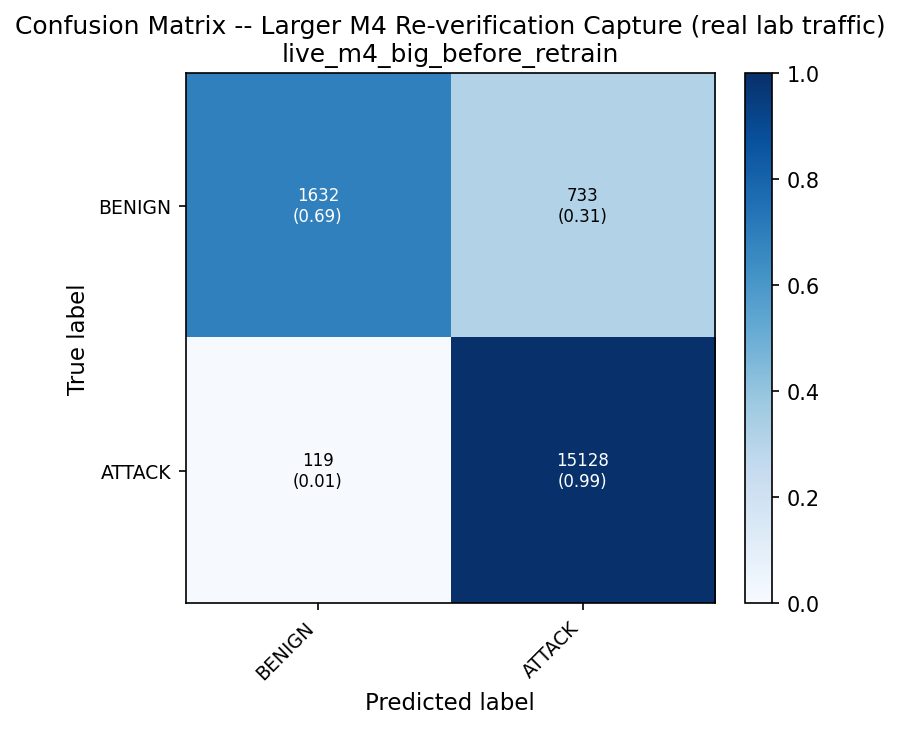
\includegraphics[width=\linewidth]{figures/finding3_confusion_before.png}
\caption{Confusion matrix, before}
\end{subfigure}
\hfill
\begin{subfigure}{0.23\textwidth}
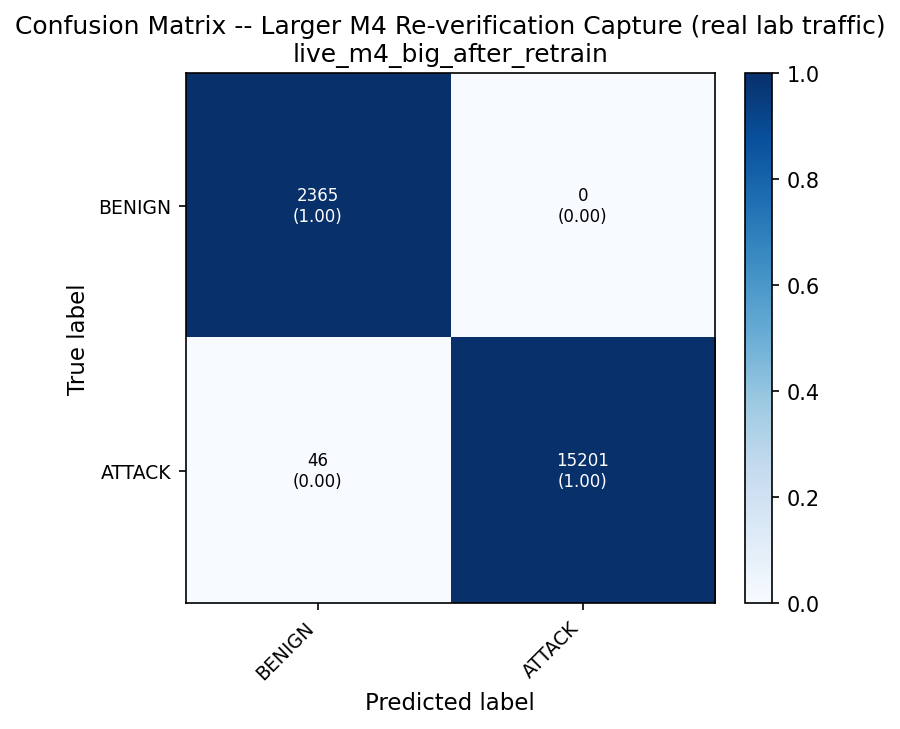
\includegraphics[width=\linewidth]{figures/finding3_confusion_after.png}
\caption{Confusion matrix, after}
\end{subfigure}
\par\bigskip
\begin{subfigure}{0.23\textwidth}
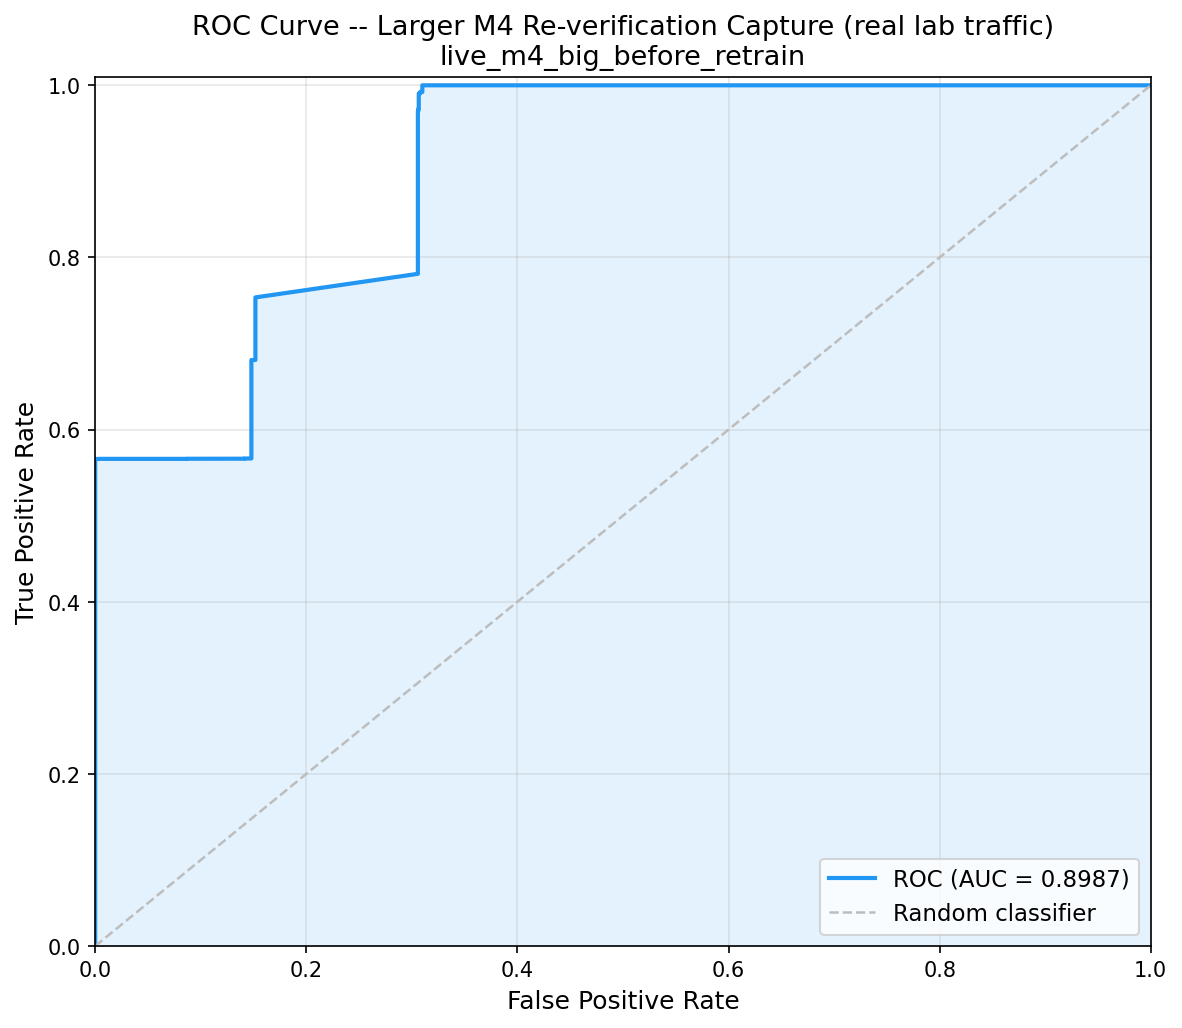
\includegraphics[width=\linewidth]{figures/finding3_roc_before.png}
\caption{ROC curve, before}
\end{subfigure}
\hfill
\begin{subfigure}{0.23\textwidth}
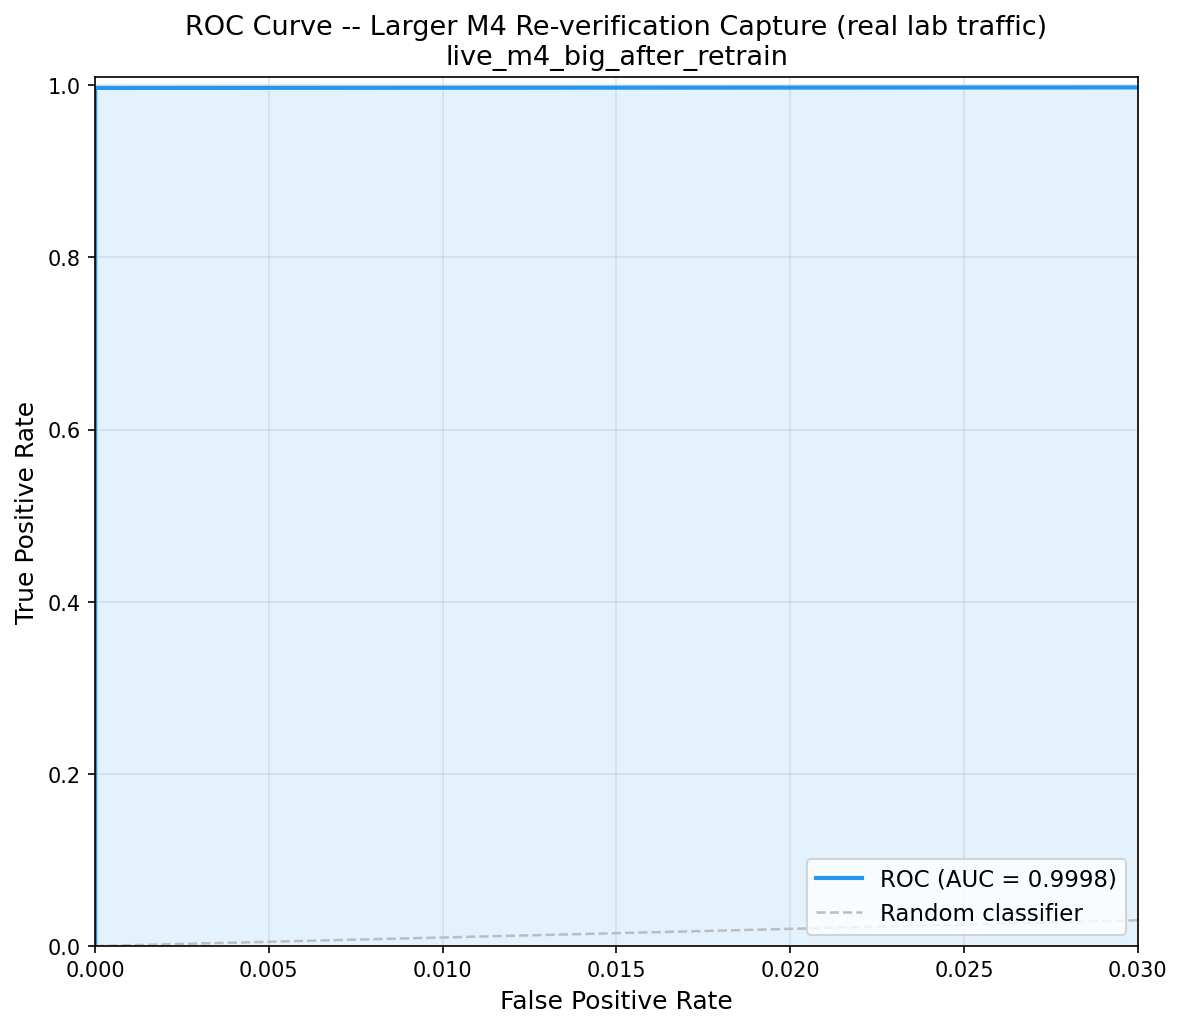
\includegraphics[width=\linewidth]{figures/finding3_roc_after.png}
\caption{ROC curve, after}
\end{subfigure}
\caption{Finding 3 (Table~\ref{tab:table4}): confusion matrices and ROC
curves before/after the second adaptive retrain, on the larger 17{,}612-flow
capture. Panel (c)'s before-retrain false positives are concentrated on the
previously-unseen port-8081 traffic.}
\label{fig:finding3grid}
\end{figure}

Table~\ref{tab:table4} and Fig.~\ref{fig:finding3grid} show the
already-corrected model scored only
95.16\% on this larger capture -- 100\% correct on the previously-seen
port~80 traffic, confirming the first fix genuinely generalized along that
axis, but 100\% \emph{wrong} on all 732 port-8081 probes, all flagged as
attacks. The first correction had learned "a single SYN with no response
is benign" as a rule specific to port~80, not a port-independent rule. A
second, targeted retrain -- manually promoted after an automated
recall-gate check rejected it on a small, noisy proxy validation sample,
a documented judgment call discussed further in
Section~\ref{sec:discussion} -- corrected this, restoring accuracy to
99.74\% with zero benign false positives across all 2{,}365 benign flows,
including all 732 previously-failing port-8081 probes. We independently
reproduced this table by replaying the original capture through the same
before/after model pair in isolation, obtaining accuracy 95.49\%/99.72\%
and ROC-AUC 0.8984/0.9998, within noise of the values above.

\begin{figure}[t]
\centering
\begin{subfigure}{0.23\textwidth}
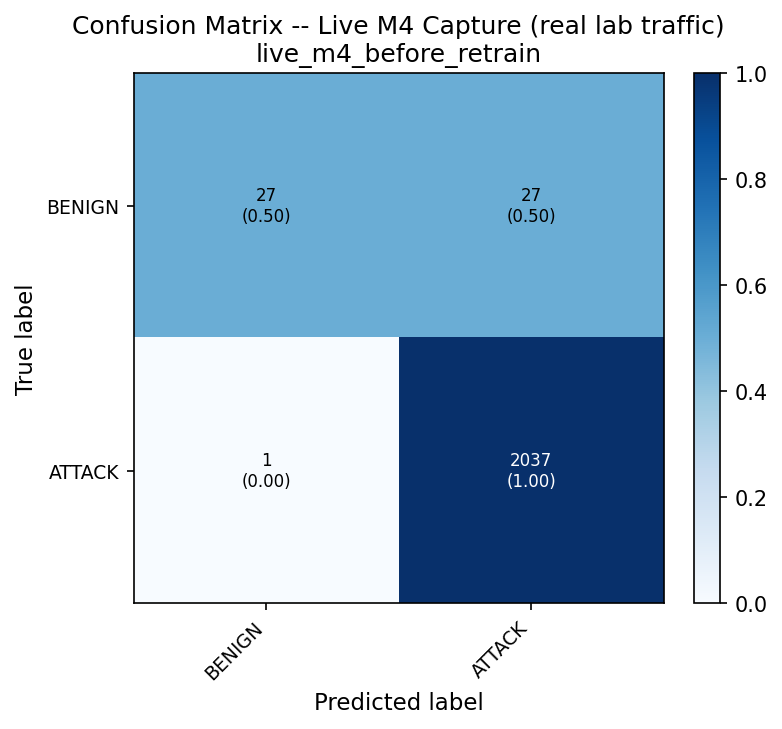
\includegraphics[width=\linewidth]{figures/finding2_confusion_before.png}
\caption{Confusion matrix, before}
\end{subfigure}
\hfill
\begin{subfigure}{0.23\textwidth}
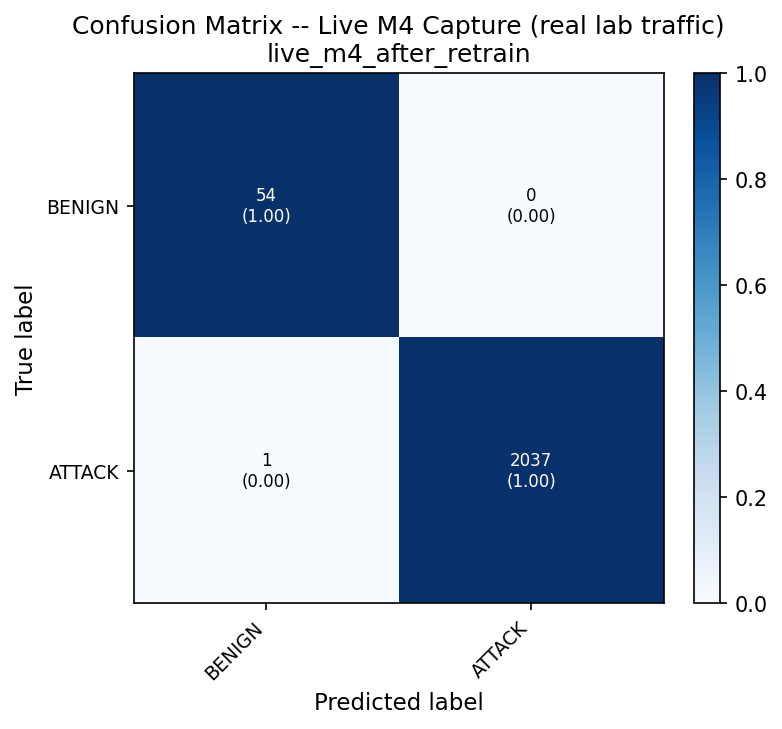
\includegraphics[width=\linewidth]{figures/finding2_confusion_after.png}
\caption{Confusion matrix, after}
\end{subfigure}
\par\bigskip
\begin{subfigure}{0.23\textwidth}
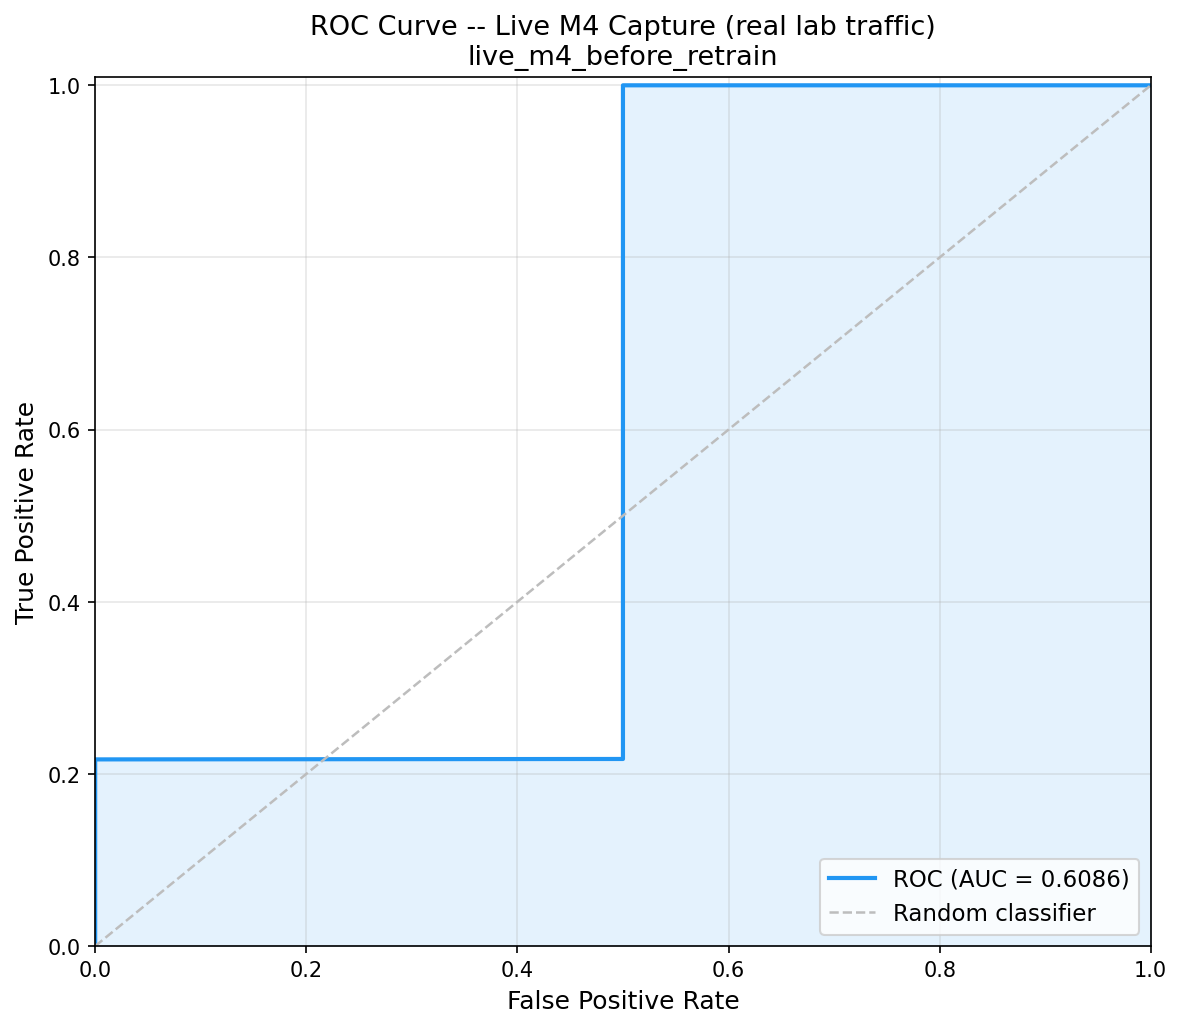
\includegraphics[width=\linewidth]{figures/finding2_roc_before.png}
\caption{ROC curve, before}
\end{subfigure}
\hfill
\begin{subfigure}{0.23\textwidth}
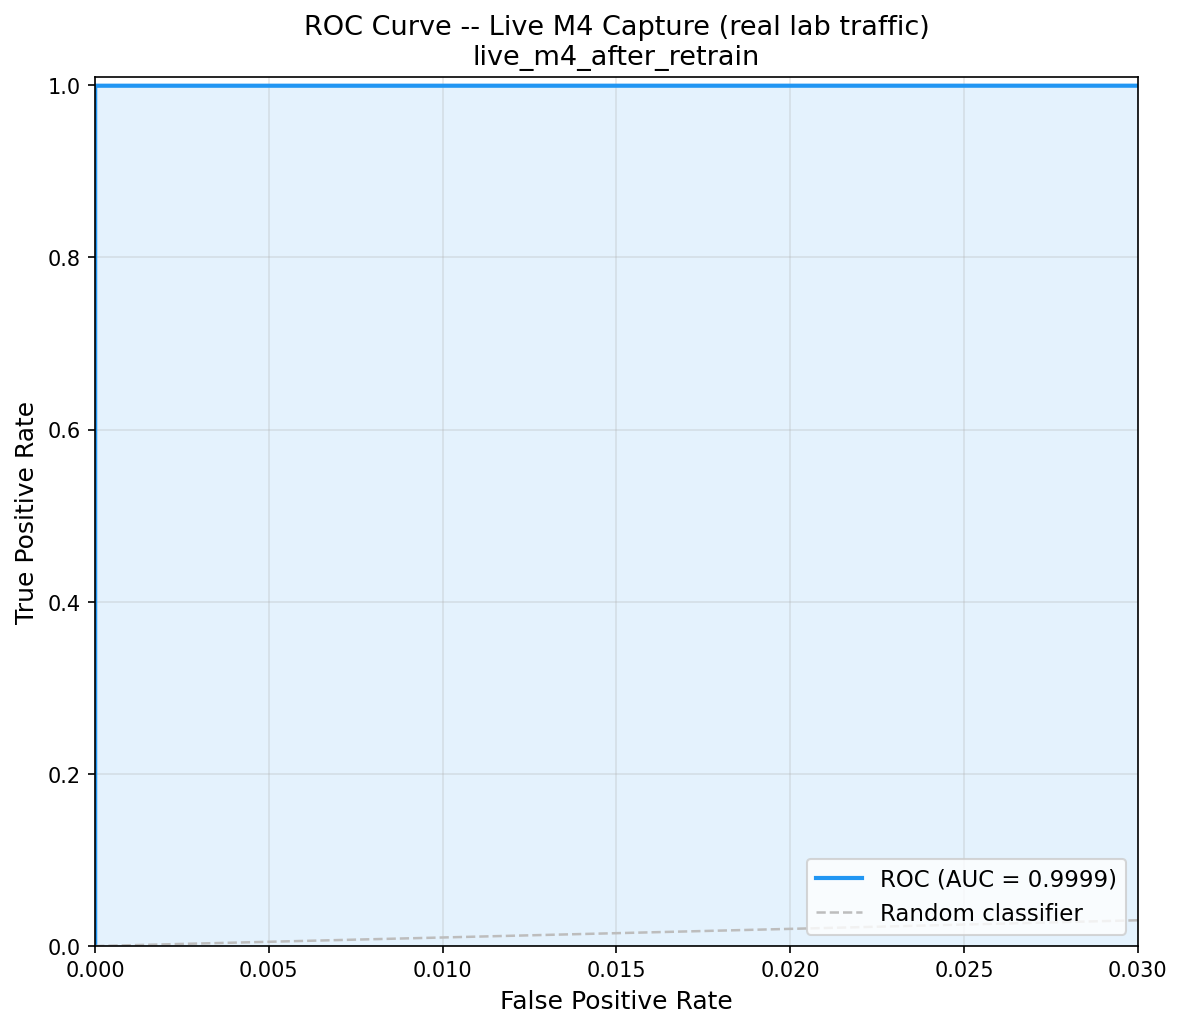
\includegraphics[width=\linewidth]{figures/finding2_roc_after.png}
\caption{ROC curve, after}
\end{subfigure}
\caption{Finding 2 (Table~\ref{tab:table3}): confusion matrices and ROC
curves before/after the first adaptive retrain. The near-diagonal
before-retrain ROC curve (c) is the visual counterpart of the ROC-AUC=0.61
in Table~\ref{tab:table3} -- the ranking was barely better than chance
despite 98.66\% accuracy.}
\label{fig:finding2grid}
\end{figure}

\begin{figure}[t]
\centering
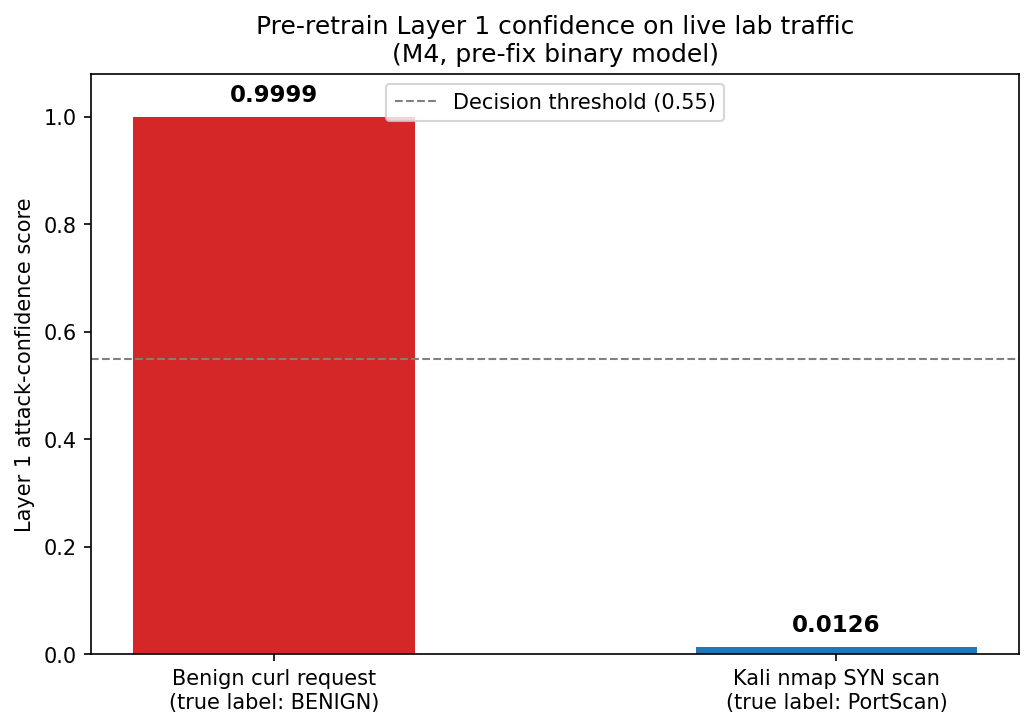
\includegraphics[width=0.9\linewidth]{figures/m4_confidence_scores.png}
\caption{Pre-fix model confidence: a benign request scored 0.9999 (confidently misclassified as attack); a real port scan scored 0.0126 (confidently misclassified as benign).}
\label{fig:m4confidence}
\end{figure}

\subsection{Feature Importance (SHAP)}

\begin{figure}[t]
\centering
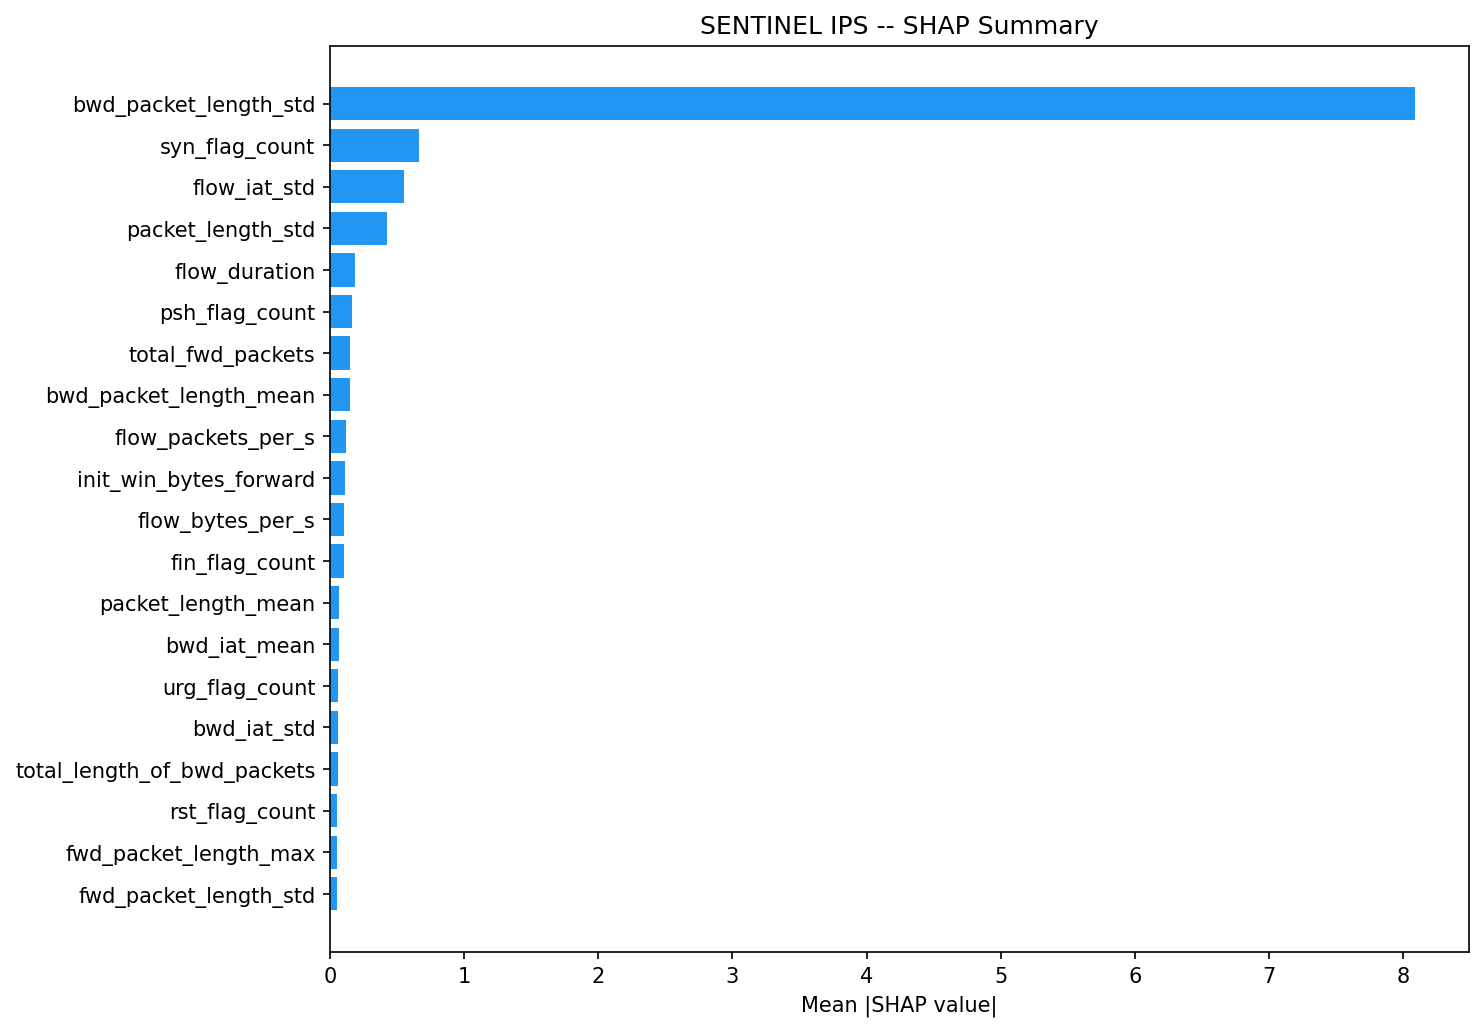
\includegraphics[width=0.95\linewidth]{figures/shap_top15.png}
\caption{Mean absolute SHAP value per feature for the CIC-IDS-2017-trained
classifier (Table~\ref{tab:table1}). \texttt{bwd\_packet\_length\_std}
dominates every other feature by close to an order of magnitude.}
\label{fig:shap}
\end{figure}

To interpret \emph{why} the classifier evaluated throughout
Section~\ref{sec:results} makes the decisions it does, we compute SHAP
values~\cite{lundberg2017shap} for the CIC-IDS-2017-trained model underlying
Table~\ref{tab:table1}. Fig.~\ref{fig:shap} shows
\texttt{bwd\_packet\_length\_std} -- the variability of backward-direction
packet sizes within a flow -- as by far the single strongest predictor,
with every other feature contributing an order of magnitude less. This is
consistent with the flows misclassified in
Section~\ref{sec:results}.B (Fig.~\ref{fig:m4confidence}): both were
minimal, near-empty exchanges with almost no backward traffic to compute
this statistic over, which is exactly the regime this dominant feature
cannot discriminate well -- a plausible mechanistic link between the
classifier's most-relied-upon feature and where it fails on live traffic.

\section{Discussion}
\label{sec:discussion}

Read together, Sections~\ref{sec:results}.A--C form a single escalating
arc. Cantone \textit{et al.}~\cite{cantone2024crossdataset} establish that
the gap exists between two curated, static datasets. We show it also
exists -- more severely -- between a curated dataset and traffic
physically captured from a live network, and, novel to this work, that it
is not closed permanently by one corrective retrain: a larger, more
diverse capture re-opens it along a dimension (destination port) the first
fix never made port-independent.

A secondary contribution is systems-level rather than purely statistical:
three previously dormant defects in the adaptive-retraining pipeline had
to be found and fixed before Table~\ref{tab:table3}'s correction could be
trusted at all. The evaluation routine originally compared retrain
candidates against misaligned feature columns, silently rejecting every
candidate regardless of quality; the retrained model's column order was
built from an unordered Python \texttt{set} intersection, silently
drifting from the order the production inference path expected; and a
documented "weight mistakes higher" retraining feature had never been
wired to the underlying classifier's sample-weighting parameter. None of
these are machine-learning failures -- they are ordinary software defects
that happened to sit directly in the path of a machine-learning
correction, and would have silently produced an apparently-successful but
actually inert retrain if left unfound.

The manually-overridden recall gate in Section~\ref{sec:results}.C is
worth stating plainly rather than hiding: an automated gate rejected the
improved candidate because its held-out CIC-IDS-2017 recall dipped
slightly on a small, noisy validation sample, even though the real-capture
result was unambiguously better. We promoted the candidate anyway, since
the live-capture evidence was the metric that mattered for the deployment
in question. This reinforces the paper's central claim from another
angle: validation gates built on benchmark-shaped assumptions about what
"improvement" looks like can themselves be miscalibrated once the target
is live traffic rather than another static split.

Gupta \textit{et al.}~\cite{gupta2025generative} address a related
adaptation problem with considerably more sophistication -- selective
sample annotation combined with generative synthesis of rare-class
examples, rather than this work's approach of mixing the entire
ground-truth capture into retraining at baseline weight. Our simpler
approach is easier for a small team to implement and audit end-to-end, but
is not sample-efficient and offers no mechanism for drift the way
generative augmentation could; Section~\ref{sec:results}.C's re-opened gap
is exactly the kind of failure a more adaptive method might have avoided
by generalizing across ports without needing to observe one directly.

\textbf{Limitations.} These findings come from a single small lab with a
specific network topology, specific attacker tooling (\texttt{nmap},
\texttt{hydra}), and one previously-unseen dimension tested (destination
port). This demonstrates that the gap persists and can re-open along at
least one untested axis; it is not proof the gap is now fully closed along
every other untested axis (protocol, traffic shape, attacker tooling).

\section{Conclusion}
\label{sec:conclusion}

We show that a network intrusion detection model achieving 99.69\%
accuracy on CIC-IDS-2017 collapsed to near-chance ranking (ROC-AUC 0.61)
against live-captured traffic from its own deployment network, was
restored via a ground-truth-informed adaptive retrain, and then partially
failed again on a larger, more diverse capture before a second correction
closed the gap. Three previously dormant defects in the correction
pipeline itself had to be fixed before this process could be trusted. The
implication for ML-IDS deployment practice is direct: benchmark accuracy
is not a reliable proxy for live performance, and validation should be
continuous and diversity-aware rather than a one-time retrain treated as a
permanent fix. Future work includes extending this analysis to the
system's multiclass attack-type classifier: in follow-on testing on this
same deployment, it showed an analogous symptom -- live detections
collapsed to a generic attack label rather than a specific one, blocking
downstream severity escalation, until a comparable corrective retrain was
applied -- suggesting the generalization gap characterized here is not
specific to binary classification, though a full characterization of that
case, to the same standard as Sections~\ref{sec:results}.A--C, is left to
future work.

\section*{Acknowledgment}
The authors thank the Department of Computer Science and Engineering,
Global Academy Of Technology, Bangalore, for their support.

\balance
\bibliographystyle{IEEEtran}
\bibliography{references}

\end{document}
